\section{Simulations}\label{sec:simulations}
\hrule

Having developed theoretical results concerning uniform inference methods for the TDNN estimator, we will proceed by testing their properties in several simulation studies.

\begin{figure}[H]
	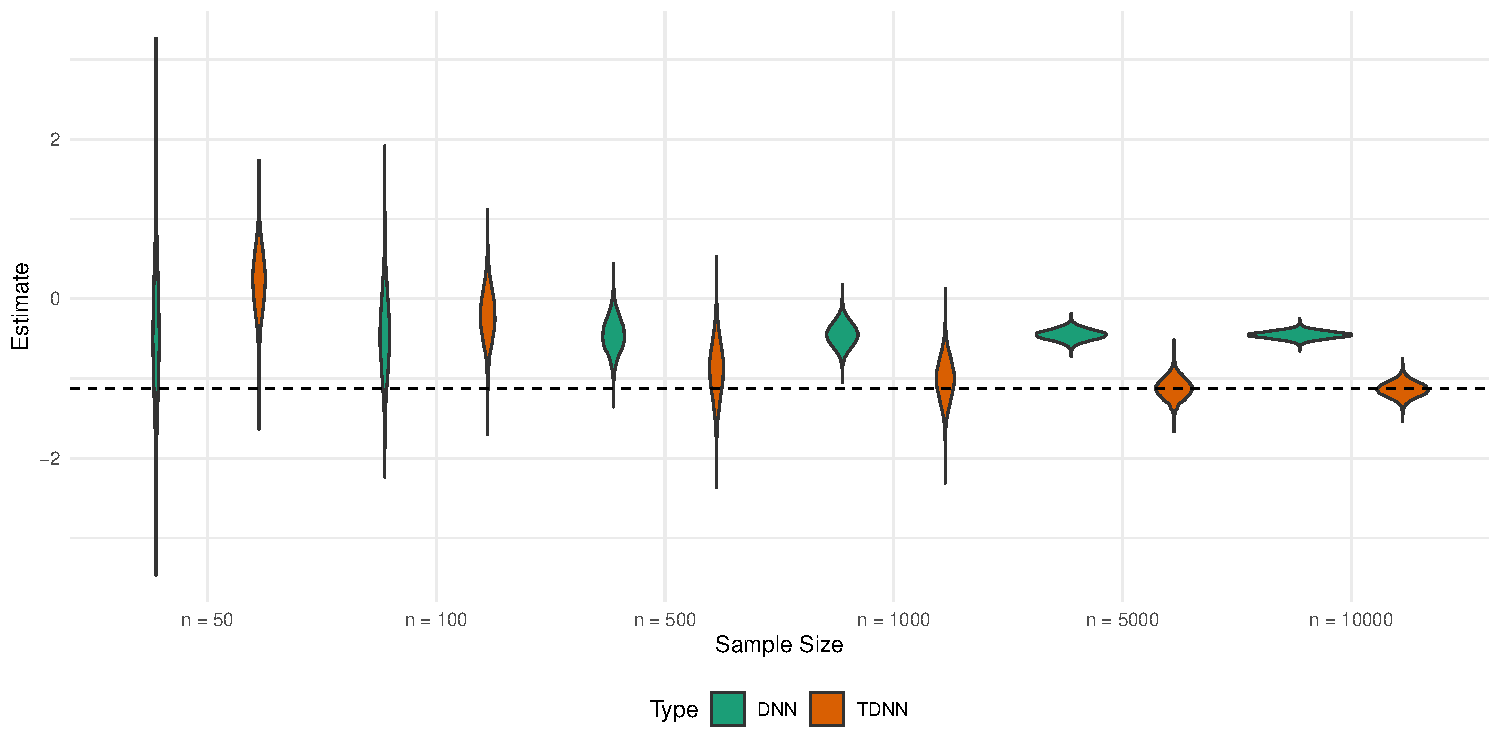
\includegraphics[width = \textwidth]{../Code/Simulations/Graphics/TDNN_DNN.pdf}
	\caption{Comparison of the DNN ($s = 20$) and TDNN ($s_1 = 20, s_2 = 50$) Estimators for different sample sizes.
		The dashed line indicates the value of the unknown regression function at the point of interest.
		Simulation Setup replicates Setting 1 from \citet{demirkaya_optimal_2024} for 10000 Monte Carlo Replications.}
\end{figure}

{\color{red} LOREM IPSUM}